\chapter{Modell und Kalibrierung}  \label{kalibrierung}

  Bildschirme und Kameras sind computergesteuerte Geräte die mit der realen Welt in Form von Licht interagieren.
  Ein Bildschirm setzt dabei seine Eingaben, das sind die Werte im \emph{Framebuffer} der Grafikkarte, in eine gewisse Strahldichteverteilung um.  
  Eine Kamera nimmt hingegen die in einem Punkt einfallende Strahldichte auf und digitalisiert sie wieder.
  Die einzelnen Pixel können dabei in beiden Fällen unabhängig angesteuert und ausgelesen werden.

  Die Zusammenhänge zwischen den digitalen und den physikalischen Werten müssen mit geeigneten Modellen beschrieben werden.
  Modelliert und rekonstruiert man die Funktionsweise der Hardware ausreichend genau, so kann man Vorhersagen über ihr Verhalten treffen.
  Damit ist es zum Beispiel möglich mit dem Bildschirm eine vorgegebene Strahldichteverteilung in einem Punkt zu erzeugen - 
  man kann ihn also zum Herstellen einer einfallenden Beleuchtung verwenden.
 
  Neben den einzelnen Komponenten muss man auch ihre Anordnung im Gesamtsystem betrachten.
  Die Beziehungen, die zwischen den Komponenten herrschen, müssen ebenfalls mit einem Modell erfasst werden.
  Für eine komplette Beschreibung müssen alle Modelle \emph{kalibriert} werden, wobei Messungen an der Hardware durchzuführen sind.
  
  Es soll nun zuerst die Gesamtanordnung aller Komponenten in Abbildung \ref{fig:setup} betrachtet werden. 
  Das System beinhaltet einen mobilen Bildschirm der zur Szene hin ausgerichtet ist und einen festen Abstand $r_l$ zum Ursprung $O$ besitzt - der Benutzer bewegt ihn wie auf einer Kugeloberfläche  rund um die Szene.
  Es gibt zwei Kameras: Eine am Bildschirm befestigte Webcam dient der Positionsbestimmung, und eine fixe DSLR-Kamera fotografiert die Szene während der Beleuchtung.
  Die Positionsberechnung der Webcam geschieht anhand von Fiducials, die so in der Welt angeordnet sind dass sie sich außerhalb der Szene befinden, aber von der Webcam gesehen werden können.
  Anhand der Webcamposition kann dann die Position des Bildschirms berechnen werden, womit sich letztendlich auch die Pixel im Raum lokalisieren lassen.
  
  Zur Durchführung dieser Arbeit wurde ein 13 Zoll Laptop mit einem TN-Bildschirm verwendet. 
  Als Webcam kam die im Bildschirm eingebaute Laptop-Kamera zum Einsatz. 
  Die genauen technischen Daten des Laptops und der verwendeten DSLR-Kamera sind im Appendix \ref{a:hardware} zu finden.

    \begin{figure}[h]
    \centering
    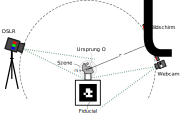
\includegraphics[width=0.7\textwidth]{../graphics/kalibrierung/setup.svg}
    \caption[Anordnung der Komponenten im System]{
    Anordnung der Komponenten im System:
  Die zu beleuchtende Szene befindet sich im Weltursprung $O$ und wird in einer abgedunkelten Umgebung von einem Bildschirm beleuchtet. 
  Die Strecke zwischen Ursprung und Bildschirmzentrum hat die Länge $r_l$, und der Szenenradius beträgt $r_s$.
  Eine am Bildschirm befestigte Webcam nimmt Bilder von geometrischen Markierungen (\emph{Fiducials}) auf, welche sich außerhalb der Szene befinden.
  Anhand der Webcambilder kann die Kameraposition, und damit auch die Bildschirmposition, berechnet werden.
  Mit einer feststehenden DSLR-Kamera werden dabei Fotos von der beleuchteten Szene gemacht.
  }
    \label{fig:setup}
   \end{figure}
 
  Die Modellierung des Systems erfolgt in zwei Teilen:
  Das \textbf{geometrischen Modell} erfasst die räumlichen Beziehungen zwischen den Komponenten und ermöglicht es die Position der Bildschirmpixel im Raum zu berechnen.
  Mit dem \textbf{radiometrische Modell} wird hingegen beschrieben, wie der Bildschirm eine Beleuchtung erzeugt, und wie die Kamera das Licht wieder aufnimmt.  
  Im Folgenden wird nun zuerst das geometrische, und dann das radiometrische Modell vorgestellt und jeweils der Kalibrierungsvorgang erklärt.
  Dabei wird unter anderem auch gezeigt wie das Gesamtsystem, ohne den Einsatz zusätzlicher Hardware, radiometrisch kalibriert werden kann.
 
 %%% aufteilung des models, ueberleitung 
 \section{Das geometrische Modell} \label{geometrisches_modell}
   
   Der geometrische Zusammenhang der Komponenten ist in Abbildung \ref{fig:geometric_model} dargestellt.
   Das Ziel des geometrischen Modells ist es, die räumliche Position der Bildschirmpixel in Abhängigkeit von der Webcamposition zu beschreiben.

   Zur Berechnung der Kameraposition wird in dieser Arbeit die Bibliothek ARToolKit \cite{artoolkit} eingesetzt. 
   Dazu muss die Geometrie der Fiducials im vorhinein bekannt sein, und der Software übergeben werden.
   Da sie im auch Vorhinein entworfen und von Hand konstruiert werden müssen, kann ihre Geometrie als bekannt angesehen werden.
   Für eine Positionsberechnung müssen desweiteren die intrinsischen Kameraparameter rekonstruiert werden (siehe Abschnitt \ref{kamera_parameter}).
   Im weiteren Verlauf wird nun davon ausgegangen, dass die Fiducial-Konfiguration und die Kameraparameter bekannt sind, und mit ARToolKit 
   die extrinsischen Parameter (Position und Rotation) der Webcam berechnet werden können.
   
   Da die Webcam fest am Bildschirm angebracht ist, lässt sich anhand der extrinsischen Parameter auch die Ausrichtung der Bildschirmebene, und damit die Pixelpositionen im Raum berchnen.
      \begin{figure}[h]
    \centering
    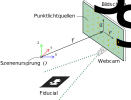
\includegraphics[width=0.6\textwidth]{../graphics/kalibrierung/geometric.svg}
    \caption[Geometrisches Modell]{ 
               Das Geometrisches Modell:
               Der Mittelpunkt der Szene legt den Ursprung $O$ des Weltkoordinatensystems fest. 
               Der Bildschirm mit den physikalischen Dimensionen $w_s$ und $h_s$ wird als eine Ebene modelliert, die durch die Vektor $\vec{f}$, $\vec{u}$ und $\vec{r}$ aufgespannt ist, wobei $\vec{f}$ die Bildschirmmitte festlegt.
               Die Pixel des Bildschirms werden als Punktlichquellen modelliert die gleichverteilt auf der Ebene liegen.
               Die Position der Webcam ist dabei realtiv zum Bildschirmzentrum definiert und die der Fiducials relativ zum Weltursprung. 
           }
    \label{fig:geometric_model}
   \end{figure}
    
    Die Translation und Rotation, die zwischen der Kamera und der Bildschirmebene besteht, muss hierzu bekannt sein, kann jedoch im allgemeinen Fall nicht von Hand bestimmt werden.
    Bei dem eingesetzten Laptop ist die Webcam zudem noch direkt im Rahmen des Bildschirms eingebaut. Maße lassen sich also nicht ohne Weiteres von Hand abnehmen.
    
    In der Praxis wurde jedoch festgestellt, dass sich das Problem dadurch sogar vereinfacht:
    Aufgrund der flachen Bauweise des Laptopbildschirms befindet sich die Blendenöffnung ungefähr in der Bildschirmebene.
    Beim Vermessen des Frustums der Laptopkamera konnte zudem herausgefunden werden, dass die optische Achse parallel zur Bildschirmnormalen ist.
    In diesem Fall ist die Sensorebene parallel zur Bildschirmebene, und die Vektoren $\vec{u}$ und $\vec{r}$  gehen direkt aus den  extrinsischen Parametern hervor.
    Zum Kalibrieren muss also lediglich die Translation der Kamera auf der Bildschirmebene gemessen werden, was leicht mit einem Lineal möglich ist.
    
  \subsection{Kamera-Parameter} \label{kamera_parameter}

%%% Pinhole Modell koalibrieren
    Beide Kameras müssen geometrisch kalibriert werden.
    Zum Einen werden die intrinsischen Parameter der Webcam für die Positionsberechnung benötigt, und zum 
     Anderen müssen die Parameter der DSLR-Kamera bekannt sein, da sie in Abschnitt \ref{display_response} zur radiometrischen Kalibrierung des Bildschirms benötigt werden.

    Für beide Kameras wird das Pinhole Modell (Abschnitt \ref{pinhole}) verwendet.
    Die intrinsischen Parameter $C$ kann man sehr einfach mit der OpenCV Bibliothek \cite{opencv} berechnen.
    Die dabei verwendete Kalibrierungsroutine basiert auf dem Algorithmus von Zhang et al. \cite{Zhang_2000}.
    Sie berechnet eine approximierte Kameramatrix anhand einem Satz Kalibrierungsbilder, die ein Schachbrett an unterschiedlichen Stellen im Kamerafrustum zeigen.
     
   Da es sich bei einer echten Kamera nicht um eine Lochkamera mit punktförmiger Blende handelt sondern ein Linsensystem zum Einsatz kommt, treten Verzerrungen im Bild auf.
   Dadurch werden gerade Linien gekrümmt auf der Sensorebene abgebildet.
   Dieser Effekt ist bei der  DSLR-Kamera aufgrund der komplizierten Linsenanordnung stärker ausgeprägt als bei der Webcam, deren Objektiv sehr simpel konstruiert ist.
   Damit eine genaue Positionsbestimmung möglich ist, muss diese Verzerrung auf jeden Fall korrigiert werden.
   Auch hierfür wird von OpenCV eine geeignete Routine zur Verfügung gestellt, mit der sich radiale und tangentiale Verzerrungen beseitigen lassen.
   
   Mit einer geometrisch kalibrierten Kamera ist es dann möglich, die  Lichtstrahlen aufzunehmen, die in einem Punkt einfallen.
   Dieser Punkt ist durch die Position der Blende im angenommenen Pinhole-Modell gegeben.
   Im den folgenden Abschnitten wird nun das radiometrische Modell behandelt, mit dem es dann möglich ist auch die Intensität dieser Lichtstrahlen in Form von Strahldichte zu messen.
    
%%%%%%%%%%%%%%%%%%%%%%%%%%%%%%%%%%%%%%%%%%%%%%%%%%%%%%%%%%%%5

 \section{Das radiometrische Modell} \label{radiometrisches_modell}
   
    Das radiometrische Modell beschreibt, wie der Bildschirm digitale Eingabedaten in Strahldichte umsetzt, und wie die Kamera sie wieder digitalisiert.
    Die Farbkanäle werden dabei im weiteren Verlauf als unabhängig betrachtet: Ein rotes Kamerapixel nimmt also nur das Licht der roten Bildschirmpixel wahr. 
    Alle hier eingeführten Definitionen und Symbole beziehen sich deshalb immer nur auf \emph{einen} Kanal, und sind auf alle drei Kanäle gleichermaßen anzuwenden.
    Der Begriff ``Pixel'' wird in diesem Abschnitt stellvertretend für ein einzelnes Subpixel verwendet.
 
    Zur Erklärung des Modells wird nun zunächst der Lichtfluss zwischen einem Pixel des Bildschirms und einem Pixel des Kamerasensors in Abbildung \ref{fig:radiometric_model} betrachtet.
    Das Licht des Bildschirms kann den Sensor entweder indirekt, über eine Reflektion an der Szene, oder aber auch direkt erreichen.
    Das direkte Licht wird nicht als Teil der einfallenden Beleuchtung angesehen,  im Folgenden wird darum bei der Modellierung ausschließlich die Strahldichte im Ursprung betrachtet.

   Damit eine praxistaugliche Modellierung möglich ist, werden mehrere Annahmen getroffen:

   \begin{description}
 
      \item[Die Beleuchtung ist distant] \hfill \\
           Das Verhältnis von Lichtquellenabstand  $r_l$ zu Szenenradius $r_s$  ist groß genug und erfüllt die Annahme einer distanten Beleuchtung.
           Damit kann die Szene im weiteren Verlauf als Punktförmig angesehen werden.
  
      \item[Pixel sind Punktlichtquellen] \hfill \\
            Die Fläche eines Pixels wird als unendlich klein angesehen und als Punktlichtquelle modelliert.  
     
      \item[$r_l$ und die Ausrichtung des Bildschirms sind festgelegt] \hfill \\
           Der Abstand $r_l$ zwischen Ursprung und Bildschirmzentrum ist festgelegt und wird immer eingehalten.
           Der Bildschirm muss außerdem immer so ausgerichtet werden, dass der Vektor $\vec{f}$ orthogonal zur Bildschirmebene steht: die Anzeigefläche ist also immer optimal zur Szene hin ausgerichtet. 
           
      \item[Der Bildschirm ist die einzige Lichtquelle] \hfill \\
           Die Aufnahmen der DSLR-Kamera sollen ausschließlich die Beleuchtung durch den Bildschirm erfassen, und dürfen nicht durch Restlicht aus der Umgebung gestört werden.
           Das kann in der Praxis durch eine zusätzliche Aufnahme (das sogenannte \emph{Darkframe}) realisiert werden.

      \item[Die Szene ist die einzige reflektierende Komponente] \hfill \\
           Das vom Bildschirm und der Umgebung reflektierte Licht wird im Modell nicht beachtet und als vernachlässigbar klein angesehen.

    \end{description}
       \begin{figure}[H]
    \centering
    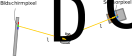
\includegraphics[width=0.6\textwidth]{../graphics/kalibrierung/radiometric_model.svg}
    \caption[Lichtfluss zwischen Bildschirm, Szene und Kamera]{ 
     Der Lichtfluss zwischen Bildschirm, Szene und Kamera:  
     Ein Lichstrahl mit der Strahldichte $l_D$ wird von einem Pixel emittiert, verläuft durch den Ursprung und erzeugt dort einen Teil der einfallende Beleuchtung.
     Ein Sensorpixel misst die Strahldichte $l_C$ von einem Lichstrahl, dessen Pfad entweder a) direkt oder b) indirekt verlaufen kann.}
    \label{fig:radiometric_model}
   \end{figure}

 
    Mit Hilfe dieser Annahmen kann die Beleuchtung die vom Bildschirm erzeugt wird durch die in den Ursprung einfallende Strahldichte beschrieben werden.
    Sie wird in dieser Arbeit mit dem Symbol $L$ bezeichnet, und als eine einfache Matrix dargestellt, in der die Strahldichte $l_D$ jedes Pixels gespeichert ist.

    Der radiometrische Zusammenhang zwischen den Bildschirm- und den Kamerapixeln wird mit eine Verkettung beider Systeme beschrieben.
    Abbildung \ref{fig:radiometric_pipeline} zeigt ihre Interaktion in Form eines Blockdiagramms.
    Beide Geräte besitzen ein Ansprechverhalten, das ganz allgemein in Form von nichtlinearen Funktionen beschrieben wird.
 
   \begin{figure}[h]
    \centering
    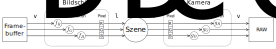
\includegraphics[width=\textwidth]{../graphics/kalibrierung/radiometric_pipeline.svg}
    \caption[Blockdiagramm der radiometrischen Beziehungen]{ 
     Blockdiagramm der radiometrischen Beziehungen: Ein Subpixel des Bildschirms setzt einen Wert $v_D$ aus dem Framebuffer der Grafikkarte in die Strahldichte $l_D$ um.
     In der Kamera wird von einem Subpixel des Sensors die Strahldichte $l_C$ wahrgenommen, und wieder in einen digitalen Wert $v_C$ umgesetzt. 
     Das Ansprechverhalten beider Geräte ist nichtlinear und wird durch eine Menge aus Funktionen beschrieben (mit $f$ und $g$ angedeutet).
     Jedes Bildschirmpixel darf dabei ein eigenes Ansprechverhalten besitzen.}
    \label{fig:radiometric_pipeline}
   \end{figure}
  
  Ist das Ansprechverhalten beider Geräte bekannt so kann man es invertieren.
  Damit ist es möglich von der Ausgabe eines Gerätes auf seine Eingabewerte zu schließen.
  Beispielsweise kann anhand eines aufgezeichneten RAW-Wertes $v_C$, auf die Strahldichte $l_C$ geschlossen werden, welche die Kamera aufgenommen hat. Man kann sie also zum Messen von Strahldichte einsetzen.
  Es kann aber auch anhand einer Strahldichte $l_D$ den zugehörigen Eingabewert $v_D$ berechnen - der Bildschirm kann also zum Erzeugen einer einfallenden Strahldichteverteilung verwendet werden.
  Damit eine Invertierung möglich ist, müssen die Ansprechkurven stetig sein, was jedoch bei Bildschirmen und Kameras aufgrund ihrer Funktionsweise angenommen werden kann.
   
%%% Channel interference
  Es ist an dieser Stelle anzumerken, dass durch die Annahme der unabhängigen Kanäle das Übersprechen zwischen den Farbkanälen des Bildschirms und den Farbkanälen der Kamera vernachlässigt wird.
  Durch das breite Frequenzspektrum der verbauten Farbfilter passiert es, dass sich beispielsweise das Licht der blauen Bildschirmpixel auch auf den Grünkanal der Kamera auswirkt.
  Dies führt zu einer verfälschten Farbwiedergabe, kann jedoch beispielsweise durch einen Weißabgleich wieder korrigiert werden \cite{Reinhard_2005}.

%%% Überleitung 
  Im Folgenden wird nun die radiometrische Kalibrierung der DSLR-Kamera beschrieben. Damit kann sie dann im Anschluss zum Messen von Strahldichte eingesetzt werden.

 \subsection{Ansprechverhalten der Kamera}  \label{dslr_calibration}  
  Das Ansprechverhalten einer Kamera beschreibt, wie die aufgenommene Strahldichte durch den Sensor und die Elektronik in einen digitalen Messwert umgewandelt wird. 
  Sind die Ansprechkurven bekannt, so kann man sie invertieren und anhand von den Kamerabildern auf die aufgenommene Strahldichte schließen. 
  Die Kamera kann also als Messgerät eingesetzt werden.
  Zusammen mit dem Pinhole-Modell ist es dann möglich, die in einem Punkt einfallende Strahldichte zu vermessen, womit es letztendlich auch möglich ist den Bildschirm radiometrisch zu kalibrieren.

%%% Einführung in Methoden
    
   Es existieren mehrere Verfahren, mit denen sich das Ansprechverhalten eines Kamera-Sensors ohne großen Aufwand bestimmen lässt. 
   Bei den Methoden von Robertson et al. \cite{Robertson_1999}, Mitsunaga et al. \cite{Mitsunaga_1999} und Debevec et al. \cite{Debevec_1997} 
   wird dazu mit einer fixen Kamera eine Reihe Bilder von einer statischen Szene geschossen, und dabei die Belichtungszeit variiert. 
   Da die vom Sensor aufgenommene relative Strahldichte proportional zur Belichtungszeit ist, kann das Ansprechverhalten rekonsturiert werden. 

%%% wie gemessen wurde
  Das Ansprechverhalten wurde in dieser Arbeit mit dem Verfahren von Robertson \cite{Robertson_1999} bestimmt. 
  Eine freie Implementierung des Robertson-Algorithmus findet sich in der Programmsammlung  \emph{pfscalibration} \cite{pfscalibration}.
  Die Pixel eines Farbkanals werden dabei als gleichwertig angesehen und es wird eine Ansprechkurve pro Farbkanal rekonstruiert.

%%% anhand von abbildung die kennlinie erklären
  In Abbildung \ref{fig:canon_response} sind die invertierten Kennlinien von dem Sensor einer Canon EOS 5D Mark II Kamera dargestellt.
  Betrachtet man die Diagramme, so fällt einem das nahezu lineare Ansprechverhalten ins Auge, das sich über den Großteil des Wertebereiches zieht.
  In den oberen Werten (>85\%), aber auch in den Schwarzwerten (<1\%) verhält sich der Sensor nichtlinear.
  Die Unterschiede in den Schwarzwerten sieht man am besten in einem Doppellogarithmischen Plot (siehe Abbildung \ref{fig:canon_response_loglog} im Anhang).
  
  \begin{figure}[h]
    \centering
    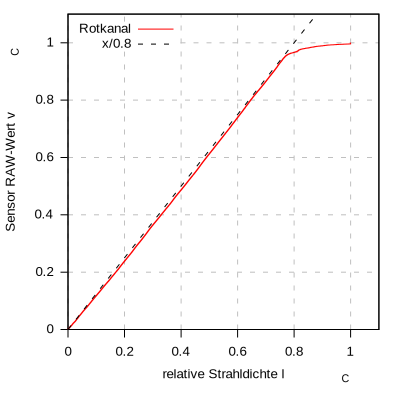
\includegraphics[width=0.3\textwidth]{../graphics/kalibrierung/canon_response_0.svg}
    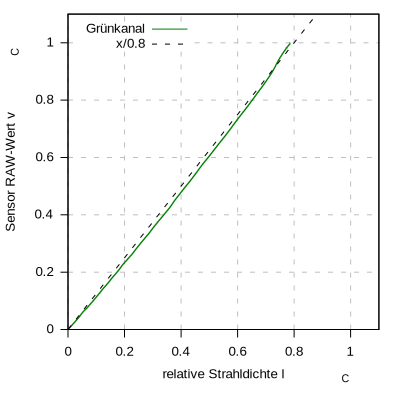
\includegraphics[width=0.3\textwidth]{../graphics/kalibrierung/canon_response_1.svg}
    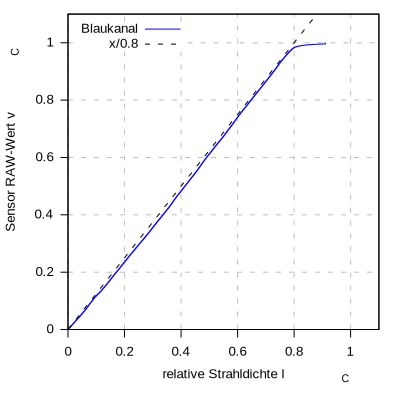
\includegraphics[width=0.3\textwidth]{../graphics/kalibrierung/canon_response_2.svg}
    \caption[Ansprechverhalten einer DSLR-Kamera]{Ansprechverhalten von dem Sensors einer Canon EOS 5D Mark II Kamera, rekonstruiert mit dem Programm pfscalibration \cite{pfscalibration}.  
    Es ist die relative Strahldichte $l_C$ über den RAW-Werten $v_C$ abgetragen, wobei beide Achsen auf den Bereich $(0,1)$ normiert sind.
 }
    \label{fig:canon_response}
   \end{figure}
  
  Mit einer radiometrisch und geometrisch kalibrierten DSLR-Kamera ist es nun möglich auch den Bildschirm zu kalibrieren.

 \subsection{Ansprechverhalten des Bildschirms}  \label{display_response}
  
  Analog zur Kennlinie einer Kamera besitzt auch ein Bildschirm ein Ansprechverhalten. 
  Mit ihm wird der Zusammenhang zwischen der Strahldichte $l_D$ eines Pixels, und dem jeweiligen Wert $v_D$ im Framebuffer beschrieben.
  Im weiteren Verlauf wird ein 24-Bit Framebuffer (8 Bit pro Farbkanal) angenommen, jedes Pixel kann also 256 unterschiedliche Werte annehmen.
 
  Das Ansprechverhalten der Pixel lässt sich durch eine Menge Funktionen
%%%% Formelle Definition des Modells 
  \begin{equation}
    l_{x,y} (v), \hspace{10mm} v \in [0,225]  
   \label{eq:display_response}
  \end{equation}
  beschreiben, wobei $(x,y)$ die Pixelkoordinate bezeichnet.
  Die Zielmenge der Funktionen ist rational, und wird jeweils durch eine minimalen Wert $l^{0}_{x,y}$, sowie einen maximalen Wert $l^{255}_{x,y}$ beschränkt.
  Dies entspricht der minimalen und der maximalen Strahldichte, die von einem Pixel ausgeht wenn man den Framebuffer 0 und 255 setzt.
 
  Da $l_{x,y}$ stetig ist kann man das inversen Ansprechverhalten
  \begin{equation}
    v_{x,y} (l) =  (l_{x,y})^{-1}(l) \hspace{10mm}  l \in [l^{0}_{x,y},l^{255}_{x,y}]
   \label{eq:inverse_display_response}
  \end{equation}
  aller Pixel berechnen. 
  Mit den invertierten Funktionen ist es dann möglich, von einer Strahldichte $l_D$ auf den Framebuffer-Wert $v_D$ zu schließen.
  
  In dieser Arbeit werden alle Ansprechkurven mit stetigen, stückweise linearen Funktionen modelliert. 
  Sie lassen sich einfach invertieren, da sie nur aus Geradenstücken bestehen: Zu jedem gegeben $l_D \in [l^{0}_{x,y},l^{255}_{x,y}]$ kann immer ein $v_D$ berechnet werden, sodass  $l_{x,y}(v_D) = l_D$.
   
  Die Funktionen $v_{x,y}$ besitzen einen eingeschränkten Definitionsbereich, der nicht für alle Pixel identisch ist. 
  Die Bereichsgrenzene $l^{0}_{x,y}$ und $l^{255}_{x,y}$  werden deshalb zusätzlich in den Matrizen $L_0$ und $L_{255}$ gespeichert:
  \begin{eqnarray}
     \forall (x,y) : \; \; \; \; \; L_0(x,y) &=& l^0_{x,y} \\
      L_{255}(x,y) & =& l^{255}_{x,y}
  \end{eqnarray}
  
  
  Im folgenden Abschnitt wird nun erklärt, wie das Ansprechverhalten  $l_{x,y}$ eines Bildschirm gemessen werden kann.
 
\subsubsection{Kalibrierungsaufbau}
  
  Den Wertebereich aller Ansprechkurven $l_{x,y}(v)$ kann man mit einer radiometrisch und geometrisch kalibrierten DSLR-Kamera messen.
  Hierzu setzt man den Framebuffer $V(x,y)$ aller Pixel auf einen bestimmten Wert und fotografiert das vom Bildschirm emittierte Licht im Ursprung.

  Da das Objektiv einer DSLR-Kamera eine große, komplizierte Linsenanordnung darstellt, kann man sie nicht ohne Weiteres von Hand so ausrichten, dass die Strahldichte im Ursprung gemessen wird.
    Es ist nicht direkt ersichtlich wo sich der Punkt befindet, durch den alle Lichtstrahlen verlaufen (siehe Kapitel \ref{pinhole}).
  
  Hier kann das Prinzip der Kamerabasierten Positionsbestimmung angewendet werden:
  Zeigt man Fiducials auf dem Bildschirm an, so kann mit ARToolKit die Position des Pinholes berechnet werden.
  Damit ist es möglich, die Kamera so auszurichten, dass sie die Strahldichte exakt im Ursprung misst.
  Eine Vorraussetzung hierfür ist, dass die intrinsischen Parameter der DSLR-Kamera für die gewählte Objektivkonfiguration bekannt sind und auch Linsenverzerrungen korrigiert werden.
  
   \begin{figure}[h]
    \centering
    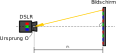
\includegraphics[width=0.6\textwidth]{../graphics/kalibrierung/radiometric_setup.svg}
    \caption[Aufbau bei der radiometrische Kalibrierung des Bildschirms]{Kalibrierungsaufbau: Eine radiometrisch und geometrisch kalibrierte DSLR-Kamera misst die von den Pixeln ausgehende, relative Strahldichte im Ursprung $O$, welcher sich im Abstand $r_l$ mittig vor dem Bildschirm befindet. 
      Die aufgezeichneten Lichtstrahlen verlassen dabei die Oberfläche unter einem bestimmten Austrittswinkel $\alpha$, der für jeden Pixel unterschiedlich ist.}
    \label{fig:radiometric_setup}
   \end{figure}
 
%%% unterabtastung von b und lineare interpolation
   Da die drei Farbkanäle als unabhängig angesehen werden, können sie alle gleichzeig mit nur einer Kameraaufnahme erfasst werden. 
 Ein Übersprechen zwischen den Kanälen wird dabei \emph{mit} aufgenommen.

   Für die Rekonstruktion von $l_{x,y}$ müssen maximal  $2^8 = 256$ Bilder aufgenommen werden.
   Der Aufwand dieser Prozedur kann durch Unterabtastung und einer geeigneten Interpolation reduziert werden.
   In dieser Arbeit werden insgesamt 33 Aufnahmen zur Rekonstruktion eingesetzt.
   Es wird dabei jeder achte Wert, einschließlich den Grenzen $V=0$ und $V=255$, vermessen und Zwischenwerte linear interpoliert.

%%% checker und pixelkorrespondenz
   Um eine Zuordnung von den Pixeln der Kalibrierungsbilder zu den Pixeln des Bildschirmes zu ermöglichen wird eine zusätzliche Aufnahme, bei unveränderter Anordnung, geschossen, wobei statt einer Graustufe ein
    Schachbrettmuster angezeigt wird.
   Anhand der Eckpunkte des Musters kann die Kameraufnahme dann durch eine perspektivische Projektion in Bildschirmkoordinaten umgerechnet werden.
   Die Genauigkeit des Messergebnisses hängt dabei von mehreren Faktoren ab, die bei der Kalibrierung unbedingt beachtet werden müssen:
  
%%% Probleme dabei
   \begin{description}

     \item[Restlicht] \hfill \\
        In der Praxis ist es nicht ohne Weiteres möglich einen Raum komplett abzudunkeln, weshalb bei der Kalibrierung auch Restlicht aus der Umgebung mit aufgenommen wird.
        Dies lässt sich durch eine weitere Aufnahme lösen, bei der die Hintergrundbeleuchtung des Bildschirms ausgeschaltet wird.
        So kann das Restlicht gezielt gemessen und von den Kalibrierungsaufnahmen abgezogen werden. 
        Diese zweite Aufnahme wird in dieser Arbeit als \emph{Darkframe} bezeichnet.

     \item[Bildrauschen] \hfill \\
        Bei der Aufnahme von Kalibrierungsdaten muss besonders auf ein gutes Signal-Rauschverhältnis geachtet werden. 
        Ist das Rauschen des Kamerasensors zu groß, so können kleinere Lichtmengen nicht mehr genau vermessen werden.
        Bildrauschen kann man zum Beispiel dadurch reduzieren, indem man Bilder mehrfach aufnimmt und den Durchschnitt bildet.

     \item[Bildschirmrand] \hfill \\ 
        Bei Messungen am Laptopbildschirm wurde festgestellt, dass die Pixel im Randbereich einen deutlich eingeschränkten Dynamikbereich besitzen:  
        Die Hintergrundbeleuchtung ist dort deutlich unregelmäßiger als in der Mitte des Anzeigefeldes, da sich dort beispielsweise die Lichtquellen befinden.
        Der Bildschirmrand eignet sich damit nur bedingt zur Beleuchtung und sollte ausgespart werden.

     \item[Aliasing] \hfill \\
        Die Oberfläche eines Flachbildschirms besitzt feine Strukturen die wesentlich kleiner sind als die Abmessungen der Subpixel selbst, wie zum Beispiel die Abstände die sich dazwischen befinden.
        Durch die hohe räumliche Frequenz kommt es beim Fotografieren zu Aliasing-Effekten. 
        Zur Abhilfe kann hier entweder ein Diffusor vor dem Bildschirm angebracht werden, oder man defokussiert die Kamera minimal.
        Beides verhält sich im Grunde wie ein Tiefpass, womit hohen Frequenzen herausgefiltert und Aliasing-Effekte eliminiert werden können. 

   \end{description} 


%%% Annahme der stetigen response curves   
  Bei der Kalibrierung wird die Annahme getroffen, dass sich das Ansprechverhalten benachbarter Pixeln nur gering unterscheidet, und über die gesamte Oberfläche betrachtet stetig verläuft.
   Unter dieser Annahme kann man die räumliche Auflösung der Kalibrierungsdaten reduzieren, wodurch sich auch das Rauschverhältnis verbessert da der Durchschnittswert vieler Pixel zur Berechnung der Ansprechkurven herangezogen werden kann.
   Dazu wird die genutzte Bildschirmoberfläche in kleine Quadratische Flächenstücke (``Patches'') eingeteilt (Abbildung \ref{fig:patches}). 
   Das Ansprechverhalten wird pro Patch berechnet, indem der Durchschnitt der darin enthaltenen Pixel gebildet wird.
   Damit kann das Sensorrauschen deutlich reduziert werden, da selbst mit sehr kleinen Patches wie beispielsweise $k=10$, schon 100 Pixel zur Berechnung eines Kurvenstützpunktes verwendet werden.
   
   Die Ansprechkurve eines einzelnen Pixels kann anschließend aus den Kurven benachbarter Patches berechnet werden, indem man sie bilinear interpoliert.
   Wie das genau funktionioniert wird in Abschnitt \ref{ldr} erklärt, da erst zur Laufzeit interpoliert wird.

   \begin{figure}[h]
    \centering
    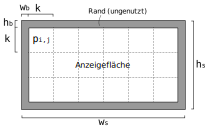
\includegraphics[width=0.6\textwidth]{../graphics/kalibrierung/patches.svg}
    \caption[Aufteilung der Bildschirmfläche]{
          Aufteilung der Bildschirmfläche: 
          Ein schmaler Rand  (grau) mit einer Höhe von $h_b$ und einer Breite von $w_b$ Pixeln bleibt wegen einem eingeschränkten Dynamikbereich ungenutzt.
          Die zur Beleuchtung verwendete Anzeigefläche (weiß) wird in quadratische Patches $p_{i,j}$ der Größe $k$ aufgeteilt (hier übertrieben groß dargestellt).
          Für jeden Patch wird ein eigenes Ansprechverhalten berechnet, indem der Mittelwert der darin enthaltenen Pixel gebildet wird.
          }
    \label{fig:patches}
   \end{figure}

  \begin{figure}[h]
   \centering
    \begin{tabular}{ccc}
%    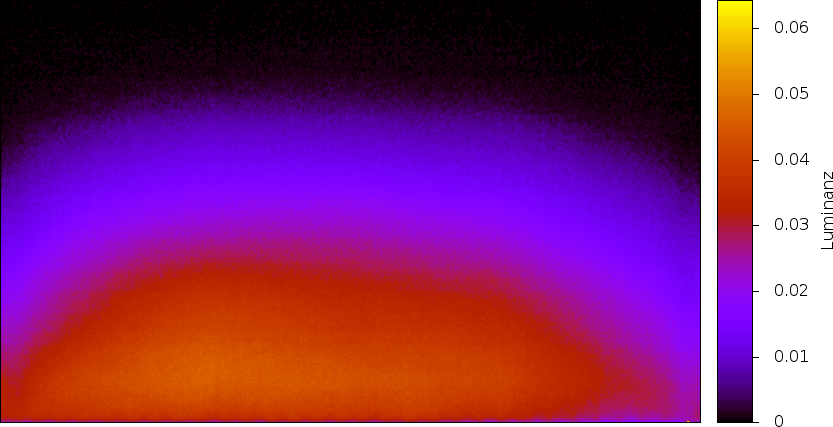
\includegraphics[width=0.3\textwidth]{../graphics/kalibrierung/backlight_close_04_map.png} &
    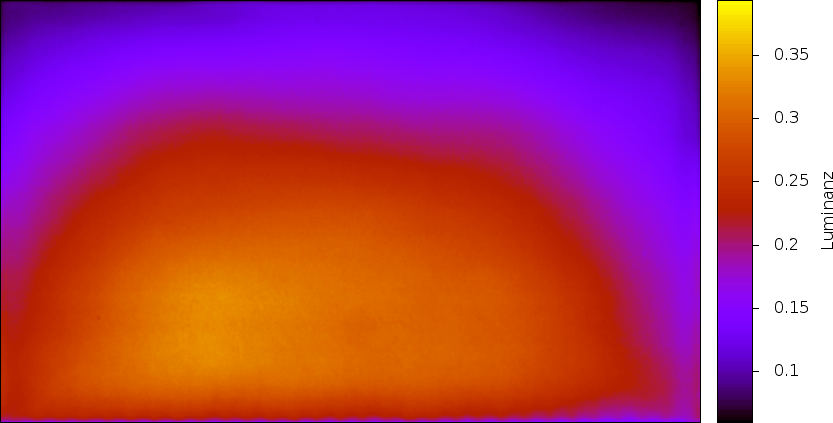
\includegraphics[width=0.45\textwidth]{../graphics/kalibrierung/backlight_close_16_map.png} &
    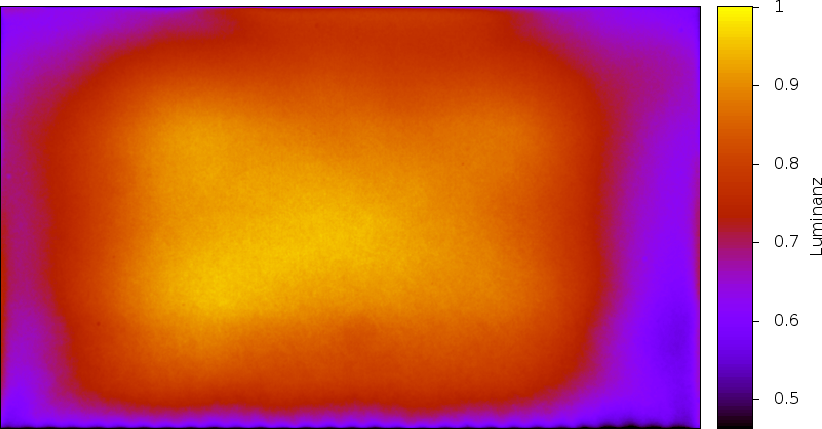
\includegraphics[width=0.45\textwidth]{../graphics/kalibrierung/backlight_close_32_map.png} \\
    
    $ V=128$ & $V=255$  \\
     
    \end{tabular}
    \caption[ Lichtverteilung des Bildschirms]{
          Die Heatmaps zeigen die gemessene Strahldichte für die mittlere ($V=128$) und die maximale Graustufe ($V=255$) der Kalibrierungsreihe. 
          Die relative Strahldichte wurde nach Gleichung \ref{eq:luminance} in Luminanz umgerechnet.
          Es fällt auf, dass sich die Lichtverteilung in beiden Aufnahmen deutlich unterscheidet -
           Der Bildschirm besitzt folglich ein, über die Oberfläche betrachtet, inhomogenes Ansprechverhalten.
 
          }
    \label{fig:lenovo_heatmap}
   \end{figure}
 

   Das Ansprechverhalten eines LCD-Bildschirms hängt sehr stark von der Richtung ab, mit der das Licht die Oberfläche verlässt.
  In Abbildung \ref{fig:lenovo_responses} ist das rekonstruierte Ansprechverhalten des Laptopbildschirms dargestellt.
   Dabei betrug $r_l =$ 50 cm und der Bildschirm wurde in 44x24 Patches der Größe $k=$30 Pixel aufgeteilt.
   Die Position eines Graphen entspricht dabei ungefähr der Position des Patches, dessen Ansprechverhalten dargestellt wird:
  Der Graph links oben zeigt die Ansprechkurven von Patch $p_{0,0}$ , welcher sich in der der linken oberen Bildschirmecke befindet. 
  Der Graph ganz rechts oben zeigt die des Patches aus der rechten oberen Ecke, und so weiter.
    
    \begin{figure}[h]
    \centering
    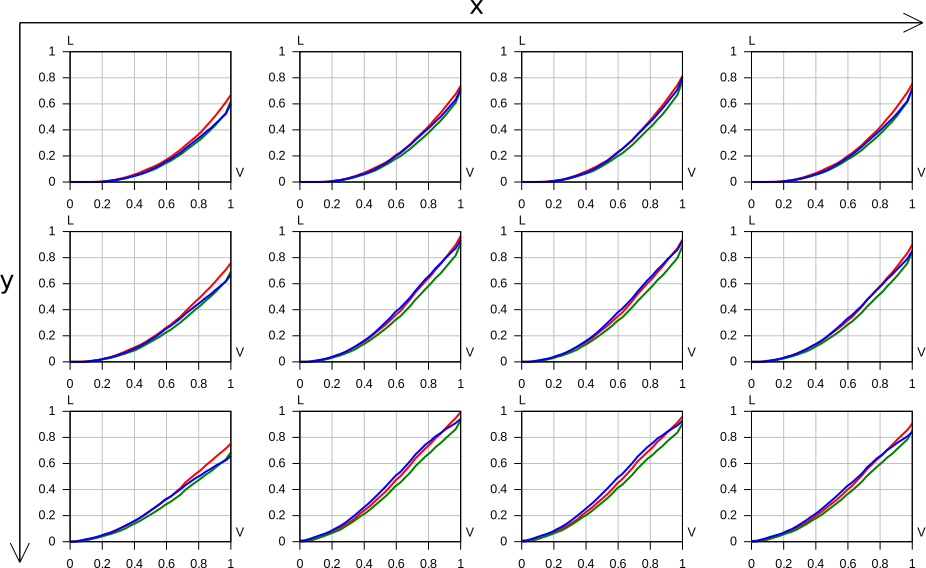
\includegraphics[width=\textwidth]{../graphics/kalibrierung/lenovo_response_multi_mod.svg}
    \caption[ Ansprechverhalten des Bildschirms]{
          Ansprechverhalten des verwendeten TN-Bildschirms:
          Zur Darstellung wurden 12 Patches gleichmäßig von der Oberfläche ausgewählt. Die Position eines Graphen entspricht der ungefähren Patchposition auf dem Bildschirm.
          Bei der Aufnahme war $r_l=50cm$, und es wurden 44x24 Patches der Größe $k=30$ Pixel verwendet (etwa 1cm groß).
          Man kann deutlich erkennen, wie der unterschiedliche Lichtaustrittswinkel das Ansprechverhalten beeinflusst:
          Mit zunehmendem Blickwinkel reduziert sich nicht nur die maximale Strahldichte, sondern es ändert sich auch das Ansprechverhalten.  
          Der Dynamikbereich ist in der Mitte des Bildschirms darum deutlich größer als im Randbereich.  
          }
    \label{fig:lenovo_responses}
   \end{figure}


